\chapter{Opgaveformulering (PO)}

%Her indsættes den konkrete opgaveformulering som I selv har udarbejdet på baggrund af et evt. projekt oplæg.

Konstruer et system der via en PC serielt kommunikerer med en hovedenhed. PCen er afhængig af et valideret login for at benytte alle funktioner. Dette login kommer fra en kodelås som har direkte kontakt til hovedenheden. Hovedenheden skal kommunikerer med nogle perifere enheder ved at benytte X10 kommunikation. Denne kommunikation skal kunne aktivere eller deaktivere ønskede 230 Vac udtag på de perifere enheder. Det skal være muligt at tilkoble en magnet lås, til en køkkenskuffe, til den perifere enhed. Der skal også være en babyalarm som registrer barnegråd. Hvis denne aktiveres skal der kunne afsendes en SMS via PCen.

Nedenstående figur \ref{fig:Systemoversigt} illustrer ovenstående.

\begin{figure}[htbp]
  \centering
    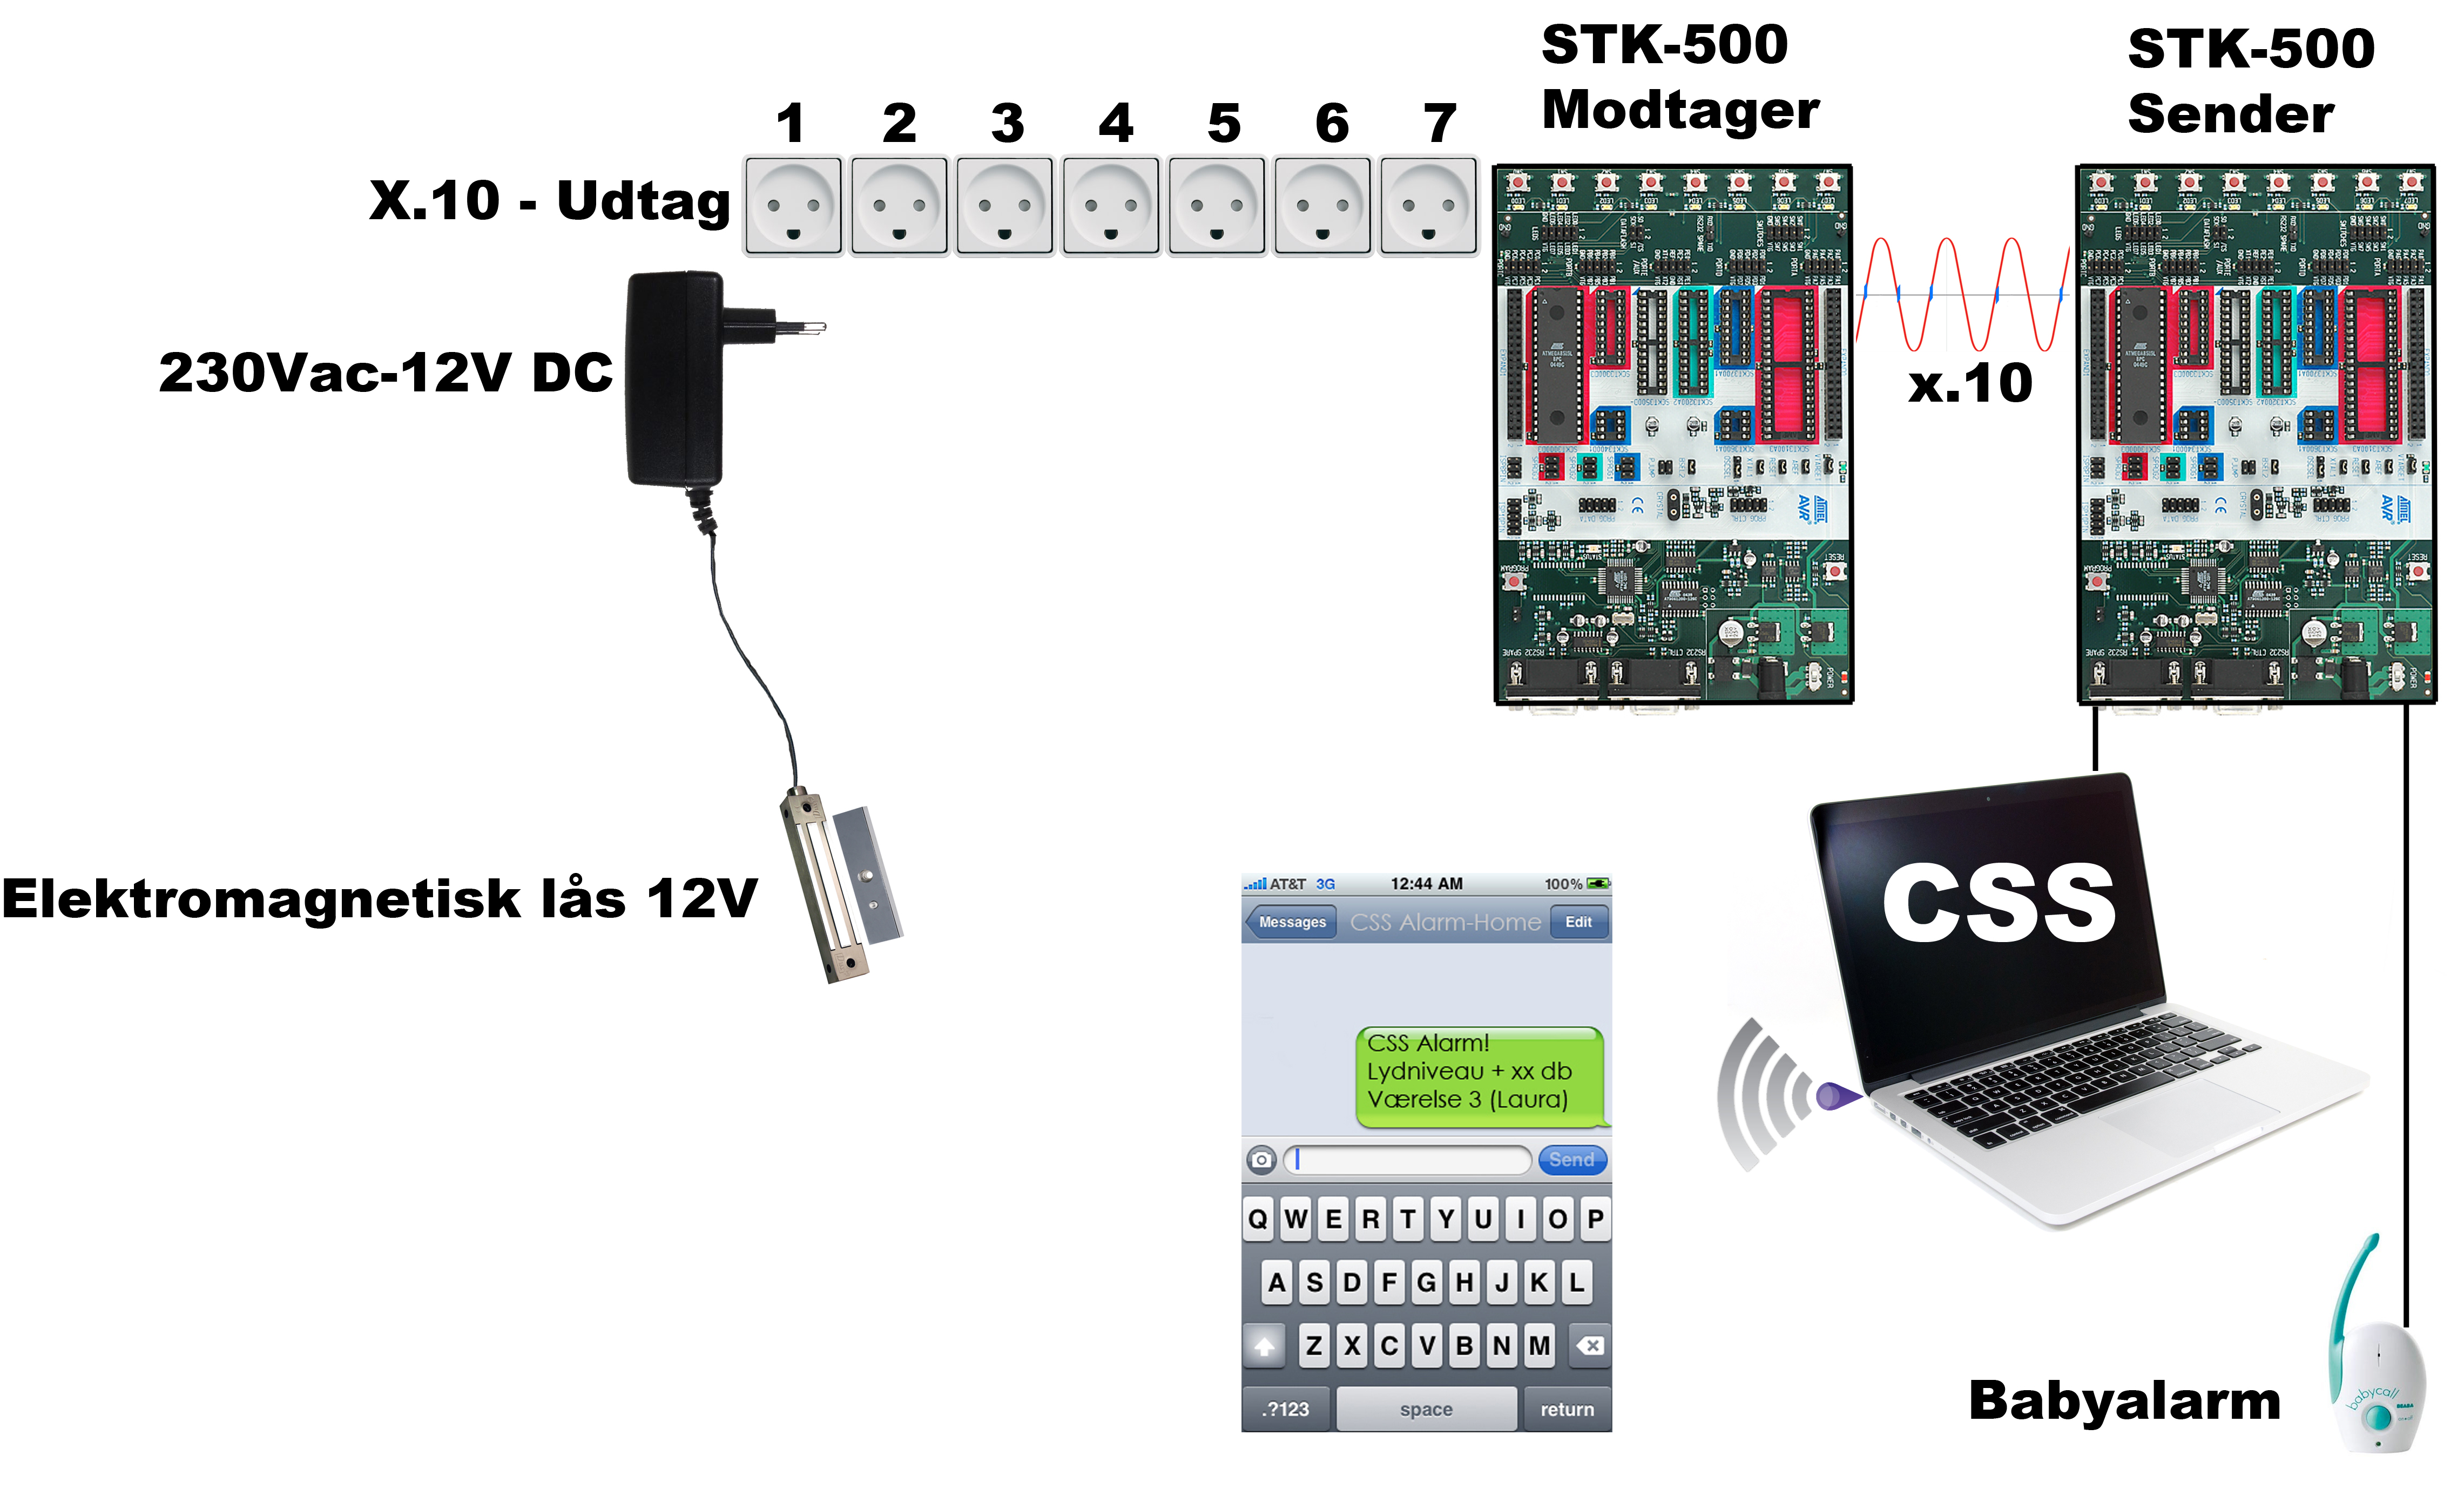
\includegraphics[width=0.8\textwidth]{billeder/Oversigt.png}
    \caption{Systemoversigt}
    \label{fig:Systemoversigt}
\end{figure}